
\documentclass[12pt,epsfig,color,russian]{article}
\usepackage[russian]{babel}
\usepackage{epsfig}
\usepackage{color}

\topmargin=0cm
\hoffset -30mm
\voffset -12mm
\setlength{\unitlength}{1mm}
\parindent=10mm
\textheight=250mm
\textwidth=190mm
\pagestyle{empty}

\begin{document}
%\begin{center}
%\huge\bf \underline{ФИЗИКА (Общая физика)}\\[5mm]
%\Large\sl Вячеслав Георгиевич ЕГОРОВ\\
%{\color{blue}(egorov@nusun.jinr.ru)}\\[10mm]
%\sf\LARGE
%2 семестр
%\end{center}
%\sf\Large
%\begin{enumerate}
%\item{\underline{\bf	Электричество и магнетизм}}

%электростатика, диэлектрики, законы постоянного тока, термоэлектри\-ческие явления, ток в электролитах и газах, маг\-нитное поле тока, откло\-нение заряженных частиц в полях, индукция, электромагнитные колеба\-ния и волны

%\item{\underline{\bf	Оптика}}

%основные свойства света, волновая оптика (поляризация, интерферен\-ция и дифракция), прохождение света через анизотропные и движущи\-еся вещества, голография, термоди\-намика излучения (световой поток, черное тело), лучевая оптика, фотоны

%\item{\underline{\bf	Атомная физика}}

%строение атомов и молекул, ионизация и диссоциация, боро\-вские орбиты, оптические переходы, правила отбора, спек\-троскопия, лазеры, лазерная спектроскопия, характеристи\-ческое рентгеновское излучение, рентгено-флуоресцентный анализ, масс-спектрометрия

%\item{\underline{\bf	Ядерная физика}}

%альфа-, бета-, гамма-процессы, ядерные реакции, взаимодействие излу\-че\-ний с веществом, детекторы ядерных излу\-чений, ядерные методы исследования материалов ("мече\-ные атомы", нейтроно-активационный анализ, ядерный ма\-гнитный резонанс)

%\end{enumerate}

%\newpage
\sf\Large
%\begin{thebibliography}{99}
%\bibitem{Фриш}
%С.Э.Фриш и А.В.Тиморева, {\bf Курс общей физики}, 2 и 3 том. {\sl\large (ГУ)}\\
%{\large
%II том: Электрические и электромагнитные явления.\\
%III том: Оптика. Атомная физика.
%}
%\bibitem{Иродов}
%И.Е.Иродов, {\bf Общая физика}. 5 томов {\sl\large (без нумерации. МИФИ.)}\\
%{\large
%{\sl Электромагнетизм. Основные законы}.\\
%{\sl Квантовая физика. Основные законы}.
%}
%\bibitem{Савельев}
%И.В.Савельев, {\bf Курс физики}. {\sl\large (3 тома. МИФИ.)}\\
%{\large
%II том: Электричество. Колебания и волны. Волновая оптика.\\
%III том: Квантовая оптика. Атомная физика. Физика твердого тела. Ядро и частицы.
%}
%\bibitem{Сивухин}
%Д.В.Сивухин, {\bf Курс общей физики}.  {\sl\large (5 томов. МФТИ, Физфак СПбГУ.)}\\
%{\large
%III том: Электричество. \\
%IV том: Оптика.\\
%V том: Атомная и ядерная физика.
%}
%\bibitem{Калашников}
%С.Г.Калашников, {\bf Электричество}.
%\bibitem{Тамм}
%И.Е.Тамм, {\bf Основы теории электричества}.
%\bibitem{Калитеевский}
%Н.И.Калитеевский, {\bf Волновая оптика}.
%\bibitem{Шпольский}
%Э.В.Шпольский, {\bf Атомная физика}.
%\bibitem{Борн}
%М.Борн, {\bf Атомная физика}.
%\bibitem{Мухин}
%К.Н.Мухин,  {\bf Экспериментальная ядерная физика}. {\sl\large (2 тома).}
%\end{thebibliography}
%\newpage
\vspace*{-20mm}
 \centerline{\underline{\huge\bf Электростатика}}\vspace{5mm}

VII B.C. греческий философ {\bf Фалес Милетский:} {\sl Янтарь, потертый о шелк, притягивает легкие предметы!}
\hfill{ }\underline{$\eta\lambda\varepsilon\kappa\tau\rho o\nu$} {\em(греч.)} = янтарь.

1600 г. английский врач {\bf William Gilbert:} {\sl То же бывает со стеклом и другими веществами!}\\
Термин ``Электризация'' (= ``янтаризация'' тел при их трении о шелк).\\

\noindent\underline{VIII век --- попытки как-то теоретически это объяснить:}
\begin{itemize}
\item
1753 г. {\bf М.Ломоносов:} электричество = быстрое вращение частичек эфира.
\item
1755 г. {\bf Л.Эйлер:} электричество = натяжение в эфире.
\item
1757 г. {\bf Ф.Эпинус:} теория "электрической жидкости" наподобие {\sl теплорода}.
\end{itemize}

\noindent\underline{а также изучение свойств электричества как физического явления:}
\begin{itemize}
\item
 1789 г. {\bf Гальвани:} физиологическое действие электричества\\ (сокращение мышц препарированной лягушки).
\item
 Электричество бывает 2 видов:
 \begin{itemize}
 \item как у стекла, потертого о кожу (+)
 \item как у кожи, потертой о стекло ($-$)
 \end{itemize}
\item
 Одноименно наэлектризованные тела отталкиваются,\\ а разноименно -- притягиваются.
\item
 При соприкосновении тел электризация\\ передается между ними\\ (как тепло, только быстрее)
\item
 1745 г. {\bf Г.В.Рихман:} \\электрический указатель (электроскоп)
 \setlength{\unitlength}{1mm}
 \begin{picture}(165,0)(0,0)
 \put(0, 0){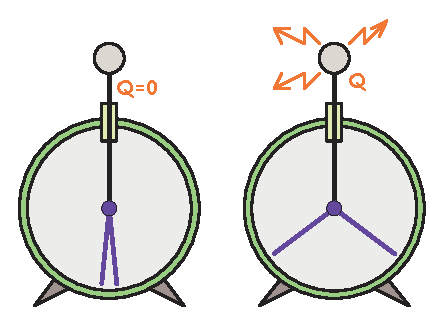
\includegraphics{GP015F01.eps}}
 \put(0,0){\makebox(0,0)[lb]{}}
 \end{picture}
\item
 Электричества разного знака друг друга компенсируют. (Если тело, заря\-женное "минусом", начать заряжать "плюсом", то его электризация сначала уменьшается до нуля, и только потом снова растет.) Гипотеза: в незаряженных телах уже $\exists$ в равных количествах и +, и $-$.
\item
Электризация {\bf наведением}: наэлектризованное тело поляризует ней\-т\-раль\-ное. Если его затем разделить, то обе половины окажутся разно\-по\-ляр\-но наэлектризованы:\\
 \setlength{\unitlength}{1mm}
 \begin{picture}(165,40)(0,0)
 \put(0, 0){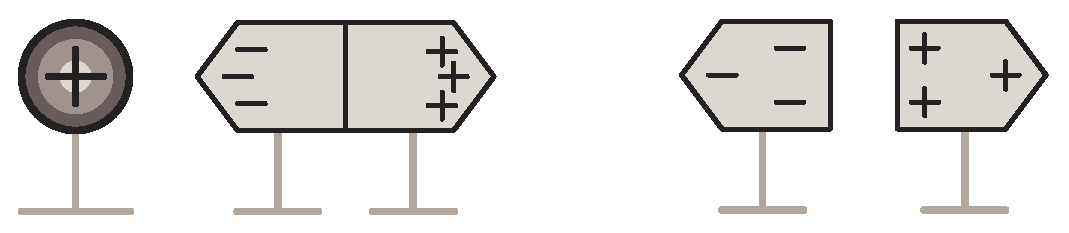
\includegraphics{GP015F02.eps}}
 \put(0,0){\makebox(0,0)[lb]{}}
 \end{picture}\\
\end{itemize}
\begin{center}
{\bf Закон сохранения электрического заряда:}\\[1mm]
\fbox{\parbox{185mm}{\color{blue}\bf Заряды не создаются и не пропадают; они лишь могут пе\-ре\-да\-вать\-ся между телами или перемещаться внутри данного тела.}}\\[1mm]
\end{center}

Теперь-то мы знаем, в чем дело. Каждый атом вещества -- это электри\-че\-ски {\bf нейтральная} система, состоящая из тяжелого ядра (+) и легких электронов ($-$). В проводниках (металлах) электроны с ядрами связаны слабо и могут дрейфовать. В изоляторах они связаны сильнее и могут только слегка смещаться (поляризация). При очень больших эл. силах изо\-ля\-тор может стать проводником (пробой). В электролитах (растворах) дви\-гать\-ся могут как легкие электроны, так и тяжелые ионы (+ и $-$).\\
 \setlength{\unitlength}{1mm}
 \begin{picture}(165,40)(0,0)
 \put(  0,0){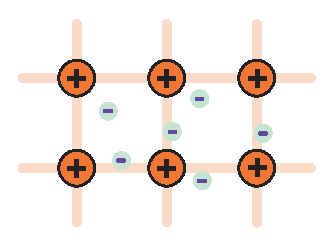
\includegraphics{GP015F3a.eps}}
 \put( 70,0){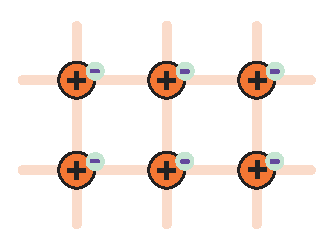
\includegraphics{GP015F3b.eps}}
 \put(140,5){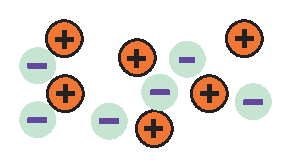
\includegraphics{GP015F3c.eps}}
 \end{picture}\\
\rule{8mm}{0mm}ПРОВОДНИК \hfill{ } ИЗОЛЯТОР \hfill{ } ЭЛЕКТРОЛИТ\rule{4mm}{0mm}\\[5mm]

{\em В действительности (узнаем это из курса ядерной физики), в ядерных реакциях с большой энергией заряженные частицы могут и рождаться, и аннигилировать, но только п\'{а}рами: сколько +, столько же и $-$. При этом сумма их с учетом знака по-прежнему остается неизменной.}


\centerline{\bf Закон взаимодействия зарядов -- ?}
Вспомним гравитацию:  $\exists$ МАССА ({\em m =  гравитационный заряд}). Разным телам мы приписываем разную массу -- $m_1$, $m_2$, ..., и они при\-тя\-ги\-ва\-ют\-ся с силой $f$, зависящей от их масс и от расстояния $r$:
\begin{displaymath}
 f=G\cdot\frac{m_1\cdot m_2}{r^2}\hspace{50mm}\vec{f}=-\vec{r}\cdot G\cdot\frac{m_1\cdot m_2}{r^3}
\end{displaymath}
Чтобы облегчить количественное описание этих сил, вводится понятие {\em сило\-вого гравитационного поля} -- то есть, пространства, в каждой точке которого на пробный гравитационный заряд $m$ действует вполне определен\-ная сила $\vec{f}=m\cdot \vec{g}$ (где $\vec{g}$ -- {\em напряженность поля}). Например, напряженность поля, создаваемого Землей у ее поверхности, направлена вертикально вниз и равна $g\simeq9.8$ м/с$^2$.

Если $\exists$ несколько зарядов,  то создаваемое ими поле подчиняются прин\-ци\-пу суперпозиции (оно равно сумме полей, создаваемых каждым зарядом по-отдельности).\\[5mm]

В электростатике вводится понятие {\em электрического заряда}. Наэлек\-три\-зо\-ванные тела имеют избыток или недостаток электронов, и $\Rightarrow$ какой-то электрический заряд $q$.

{\em Точечный} заряд $q$ отталкивается от другого {\em точечного} заряда $Q$ (если их знаки одинаковы) или притягивается к нему (если их знаки различны)\\
 \setlength{\unitlength}{1mm}
 \begin{picture}(165,25)(0,0)
 \put(  20,0){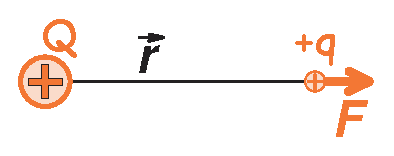
\includegraphics{GP015F4b.eps}}
 \put( 120,0){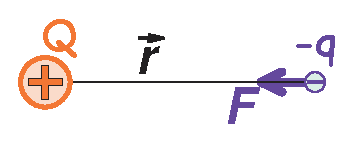
\includegraphics{GP015F4c.eps}}
 \end{picture}\\
Закон, открытый Шарлем Кулоном (Charles-Augustin de Coulomb) в 1785 г:
\begin{displaymath}
 f=k\cdot\frac{Q\cdot q}{r^2}\hspace{50mm}\vec{f}=\vec{r}\cdot k\cdot\frac{Q\cdot q}{r^3}
\end{displaymath}
Что принять за единицу заряда? Для этого положим $k\equiv1$. Например, в CGS-системе это -- такой точечный заряд, который взаимодействует с равным ему точечным зарядом, находящимся на расстоянии 1 см, с силой в 1 дину. В электротехнике другая единица: 1 Кулон (1 Кл) = 3$\cdot10^9$ CGSE.\\
 \setlength{\unitlength}{1mm}
 \begin{picture}(190,70)(0,0)
 \put(  140,0){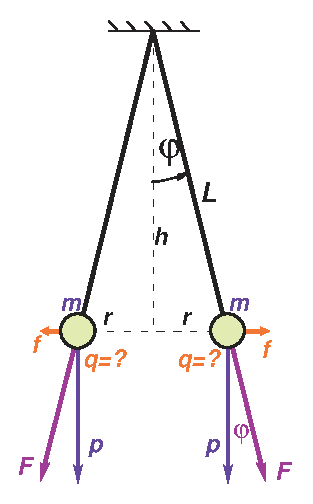
\includegraphics{GP015F05.eps}}
 \put(0,80){\makebox(0,0)[lt]{\parbox{145mm}{\underline{Задачка:} Два одинаково заряженных шарика по 0.1 г на ниточках по 25 см разошлись на расстояние 2$r$=5 см. Каков их заряд?\\
 \underline{Решение:} Сила отталкивания $f=q^2/(2r)^2$.\\
 Равновесие -- когда ранодействующая сила\\ $\vec{F}=\vec{p}+\vec{f}$ направлена
 вдоль нити.
 }}}
 \put(0,0){\makebox(0,0)[lb]{\parbox{140mm}{Из подобия треугольников при малом $\varphi$ получаем:
 \begin{displaymath}
 \frac rL\simeq\frac rh=\frac fp=\frac{q^2}{mg(2r)^2}
 \end{displaymath}
 }}}
 \end{picture}\\
Откуда находим заряд в единицах CGSE:
\begin{displaymath}
 q=2r\cdot\sqrt{\frac{mgr}L}=5\cdot\sqrt{\frac{0.1\cdot 981\cdot 2.5}{25}}\simeq 15.6 \;\;{\rm CGSE}\hspace{5mm}
 (=5.2\cdot10^{-9}\;K)
\end{displaymath}
\vspace*{5mm}

Для облегчения количественного описания сил между зарядами в элек\-т\-ро\-ста\-тике тоже вводится понятие {\em силового поля}. Что это такое?\\
 \begin{picture}(190,35)(0,0)
 \put(110,0){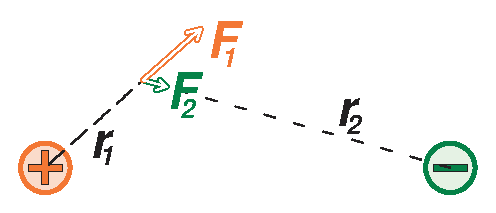
\includegraphics{GP015F06.eps}}
\put(0,0){\makebox(0,0)[lb]{\parbox{105mm}{
 Пусть имеется какая-то система зарядов. Для изучения ее свойств будем помещать в каждую точку \underline{\em пробный заряд q} и смотреть, какая сила $\vec{F}$ на него действует. }}}
 \end{picture}\\
 Этот пробный заряд должен быть:
\begin{itemize}
\item Маленький -- чтобы он собою не искажал изучаемую систему;
\item Точечный -- чтобы было проще;
\item Положительный -- просто для определенности.
\end{itemize}
По закону Кулона сила $\vec{F}$ всегда будет пропорциональна заряду $q$, поэтому лучше приводить не саму эту силу, а ее отношение к заряду $q$ -- {\em ``удельную силу''} или, иначе, \underline{\em НАПЯЖЕННОСТЬ} $\vec{E}\equiv\vec{F}/q$. Таким образом, мы в каждой точке найдем $\vec{E}$ и тем самым определим силовое {\em электрическое поле}, создан\-ное системой зарядов. Теперь можно про заряды забыть, а говорить о свойствах поля.

Кроме напряженности полезно ввести понятие \underline{\em силовой линии} -- такой линии, в каждой точке которой напряженность направлена по касательной.\\
 \begin{picture}(190,35)(0,0)
 \put(40,0){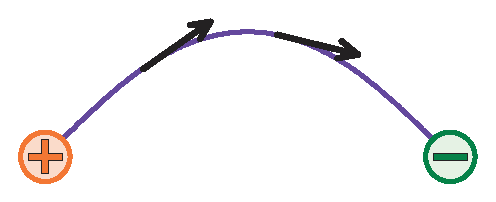
\includegraphics{GP015F07.eps}}
 \end{picture}\\

 Точечный заряд создает сферически-симметричное поле:\\
 \begin{picture}(190,70)(0,0)
 \put(10,0){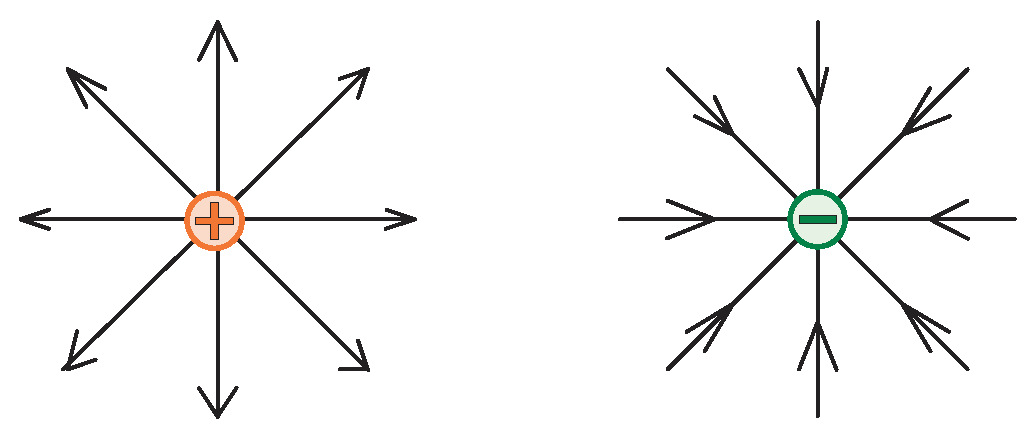
\includegraphics{GP015F08.eps}}
 \end{picture}\\

 Поле двух разноименных зарядов (диполь):\\
 \begin{picture}(190,80)(0,0)
 \put(30,0){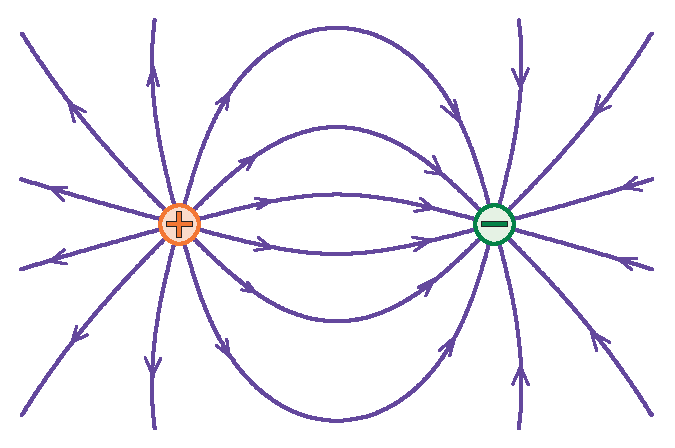
\includegraphics{GP015F09.eps}}
 \end{picture}\\


\newpage
Силовые линии -- это условность. На самом деле нет там никаких линий! Сколько их нарисовать -- наше дело.

Давайте условимся: чем больше НАПРЯЖЕННОСТЬ -- тем ГУЩЕ рисуем линии.\\
 \begin{picture}(190,60)(0,0)
 \put(20,0){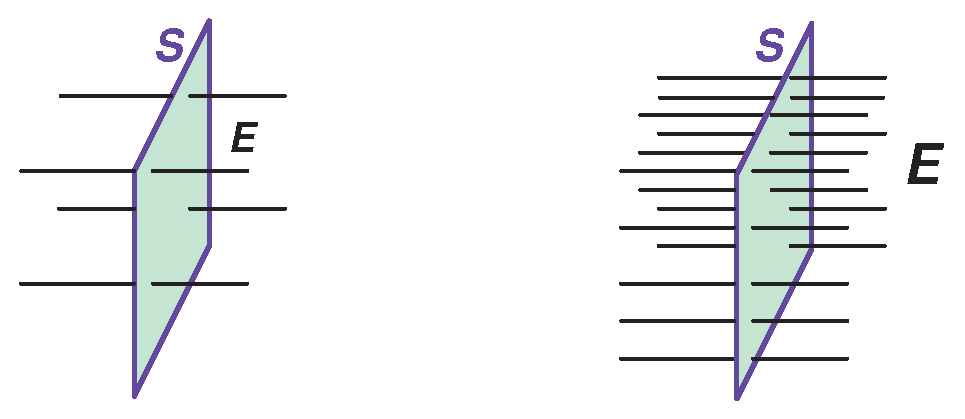
\includegraphics{GP015F10.eps}}
 \end{picture}\\
Более того, давайте условимся, чтобы число линий $N$ через площадку $S$ численно равнялось напряженности $E$:
\begin{displaymath}
\frac{N}{S}=E\hspace{20mm}\lim_{\Delta S\rightarrow0}\frac{\Delta N}{\Delta S}=E\hspace{20mm}\frac{d N}{d S}=E
\end{displaymath}
Если $E$ не перпендикулярна поверхности $S$, то надо брать только ее нор\-маль\-ную составляющую $E_n=E\cdot \cos\alpha$.\\
 \begin{picture}(190,55)(0,0)
 \put(0,0){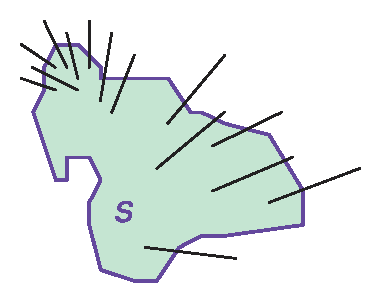
\includegraphics{GP015F11.eps}}
\put(60,0){\makebox(0,0)[lb]{\parbox{130mm}{
Таким образом, если в электрическом поле $\exists$ какая-то поверхность $S$, то общее количество силовых линий $N$, пересекающих эту поверхность, (т.е., ПОТОК НАПРЯЖЕННОСТИ), будет равен
\begin{displaymath}
N=\int\limits_S E_n dS
\end{displaymath}
}}}
 \end{picture}\\
Рассмотрим точечный заряд $q$. Сколько линий из него выходит? Проведем (мысленно) вокруг него сферу радиуса $R$. Тогда, по закону Кулона, на поверхности сферы $E=q/R^2$ (причем $\vec{E}\perp$ поверхности), площадь сферы $S=4\pi R^2$, а число линий $N=4\pi q$.

\begin{center}Теорема Остроградского-Гаусса:\\
\fbox{\parbox{188mm}{\color{blue}\bf Поток напряженности через любую замкнутую поверхность равен произведению 4$\pi$ на сумму охватываемых зарядов.}}
\end{center}

Доказательство: рассмотрим замкнутую поверхность, внутри которой $\exists$ заряд $q$\\
 \begin{picture}(190,35)(0,0)
 \put(40,0){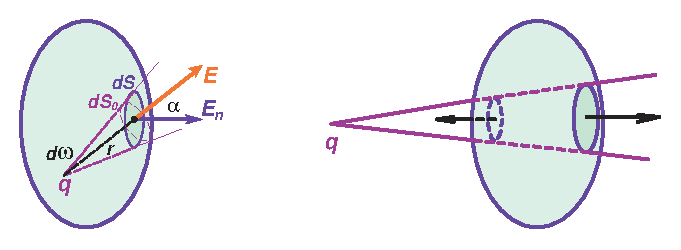
\includegraphics{GP015F12.eps}}
 \end{picture}\\
Поток напряженности через малую площадку $dS$ равен
\begin{displaymath}
 dN = E_n\;dS \;=\; E\;\cos\alpha\;dS\;=\;E\;dS_0\;=\;\frac{q}{r^2}\;dS_0\;=\;\frac{q}{r^2}\;r^2\;d\omega\;=\;q\;d\omega
\end{displaymath}
Полный поток напряженности через всю поверхность $S$ равен
\begin{displaymath}
 N\;=\;\oint\limits_S dN\;=\;q\;\oint\limits_S d\omega\;=4\pi q
\end{displaymath}
Если заряд $q$  $\exists$ вне замкнутой поверхности, то при интегрировании $\forall\;d\omega$ войдет дважды: один раз на входе в поверхность (со знаком $-$), а второй раз -- на выходе (со знаком +), и в итоге $N=0$.\\

\underline{\bf Применение теоремы Остроградского-Гаусса}
\begin{itemize}
\item{\bf Поле равномерно заряженной $\infty$ плоскости.}\\
 \begin{picture}(170,50)(0,0)
 \put(-5,0){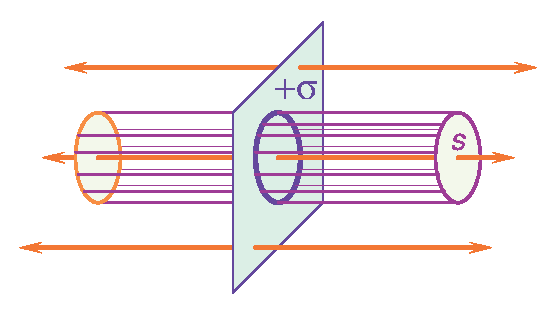
\includegraphics{GP015F13.eps}}
 \put(90,-5){\makebox(0,0)[lb]{\parbox{90mm}{
 Пусть плотность заряда $\frac{\partial q}{\partial S}=+\sigma$. Ясно, что $\vec{E}$ везде $\perp$ плоскости; но какова ее величина? Выделим цилиндрический объем и найдем поток напряженности через его торцы (чезез боковую поверхность поток =0, т.к. $\vec{E}\parallel$ ей):
 }}}
 \end{picture}\\
\begin{displaymath}
N=N_1+N_2=ES_1+ES_2=2ES
\end{displaymath}
А по теореме О-Г, поток = $N=4\pi q=4\pi S\sigma$. Сравнивая, получаем:
\begin{displaymath}
2ES=4\pi S\sigma\hspace{20mm}\Rightarrow\hspace{20mm}E=2\pi\sigma
\end{displaymath}
Не зависит от расстояния до плоскости!!!
\item{\bf Поле двух равномерно заряженных $\infty$ плоскостей.}\\
 \begin{picture}(170,50)(0,0)
 \put(-10,0){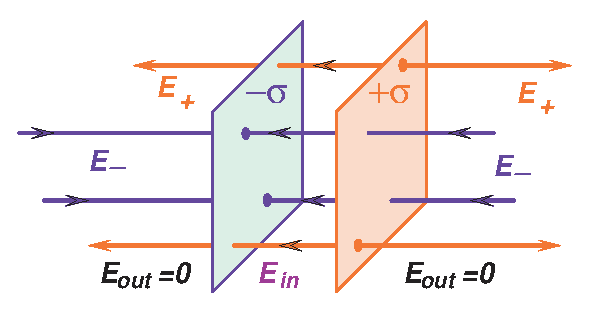
\includegraphics{GP015F14.eps}}
 \put(90,-5){\makebox(0,0)[lb]{\parbox{90mm}{
 Плоскости заряжены одинаково, но разным знаком. Одна созда\-ет поле $\vec{E_+}$, другая -- поле $\vec{E_-}$. Вне пластин поля направлены в разные стороны, и они компенсируют друг друга:
 \begin{displaymath}
 \vec{E}_{\rm out}=\vec{E}_++\vec{E}_-=0\;,
 \end{displaymath}
 }}}
 \end{picture}\\
а между пластин направления полей совпадают, и они суммируются:
 \begin{displaymath}
 \vec{E}_{\rm in}=\vec{E}_+ +\vec{E}_- = 2\cdot 2\pi\sigma = 4\pi\sigma
 \end{displaymath}
\item{\bf Поле равномерно заряженной сферы.}\\
 \begin{picture}(170,80)(0,0)
 \put(-10,0){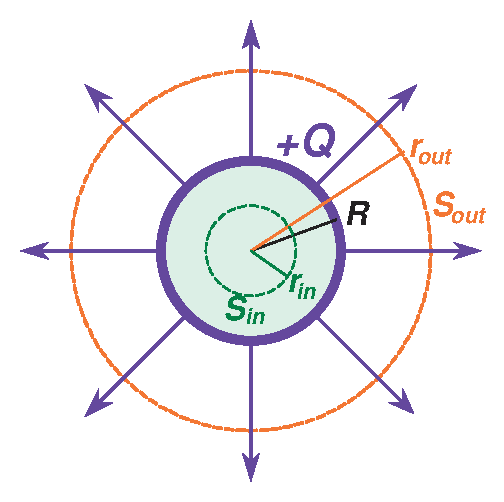
\includegraphics{GP015F15.eps}}
 \put(75,0){\makebox(0,0)[lb]{\parbox{105mm}{
 Сфера радиуса $R$ имеет равномерно рас\-пре\-де\-ленный по поверхности заряд $Q$. Ясно, что поле везде направлено $\parallel$ ра\-ди\-у\-су. Мыс\-лен\-но проведем сферу с радиусом $r_{\rm out}$. Ее площадь $S_{\rm out}=
 4\pi r_{\rm out}^2$, поле $\vec{E}_{\rm out}$ везде $\perp$ ее поверхности, и по теореме О-Г:
 \begin{displaymath}
 E_{\rm out}\cdot S_{\rm out}= 4\pi Q
 \end{displaymath}
 откуда получаем, что поле $E_{\rm out}=Q/r_{\rm out}^2$ (как если бы заряд $Q$ был точечным).
 }}}
 \end{picture}\\
 ВНУТРИ сферы (при $r_{\rm in}<R$) по теореме О-Г $E_{\rm in}\!\cdot\! S_{\rm in}=0$, и поля НЕТ.
\item{\bf Поле равномерно заряженного шара.}\\
 Если заряд $Q$ распределен не по ПОВЕРХНОСТИ сферы, а по всему ее внутреннему ОБЪЕМУ, то внешнее поле будет таким же: $E_{\rm out}=Q/r_{\rm out}^2$. А вот внутреннее (при $r_{\rm in}<R$) будет по теореме О-Г определяться  не всем зарядом $Q$ только той его частью $q$, которая находится ВНУТРИ воображаемой сферы радиусом $r_{\rm in}$. Поскольку эта часть $\propto$ объему $V_{\rm in}=\frac43\pi r_{\rm in}^3$, то $q=Q\cdot\left(r_{\rm in}/R\right)^3$, и поле $E_{\rm in}=q/r_{\rm in}^2=Q\cdot r_{\rm in}/R^3$.\\
 \begin{picture}(170,30)(0,0)
 \put(-5,0){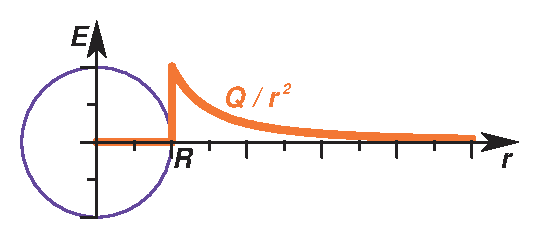
\includegraphics{GP015F16.eps}}
 \put( 90,0){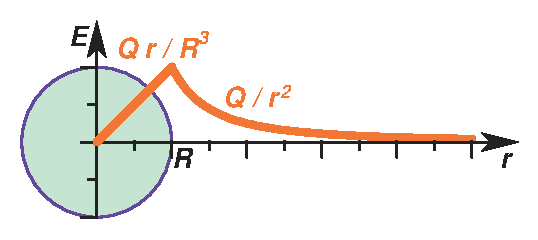
\includegraphics{GP015F17.eps}}
 \end{picture}\\
\item{\bf Поле равномерно заряженного $\infty$ цилиндра.}\\
 \begin{picture}(170,75)(0,0)
 \put(-10,0){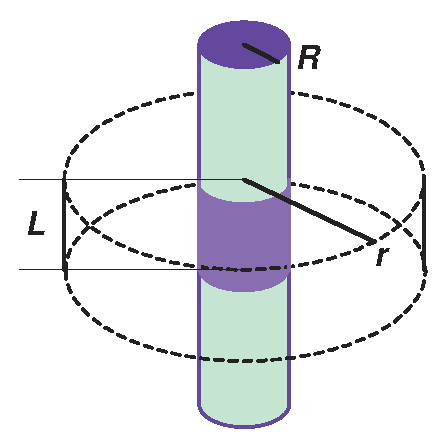
\includegraphics{GP015F18.eps}}
 \put(65,0){\makebox(0,0)[lb]{\parbox{115mm}{
 по цилиндру с радиусом $R$ распределен заряд с поверхностной плотностью $\frac{\partial q}{\partial S}=+\sigma$. Поле $E$ на расстоянии $r>R$ от оси цилиндра найдем, проведя воображаемый цилиндр с таким же радиусом и высотой $L$. Поток напряженности через торцы = 0 (поле $\perp$ оси), а через боковую поверхность --- $N=S\cdot E=2\pi r L \cdot E$. Заряд внутри цилиндра: $q=\sigma\cdot 2\pi R L$. Но по теореме О-Г должно быть $ N= 4\pi q$, поэтому
 }}}
 \end{picture}\\[-5mm]
 \begin{displaymath}
2\pi r L \cdot E = 4\pi\sigma\cdot 2\pi R L\hspace{20mm}\Rightarrow\hspace{20mm}E=4\pi\sigma\;\frac{R}{r}
 \end{displaymath}
Внутри же заряженного цилиндра (как и в случае со сферой) поле = 0.
\end{itemize}
\vspace*{10mm}

\underline{\bf Работа электрических сил.}\\
 Пусть в поле заряда $Q$ из точки A в точку B перемещается заряд $q$, проходя\\
  \begin{picture}(170,70)(0,0)
 \put(0,0){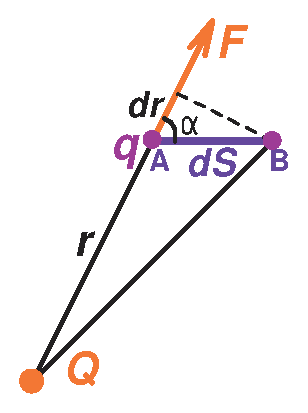
\includegraphics{GP015F19.eps}}
 \put(55,0){\makebox(0,0)[lb]{\parbox{135mm}{
  малый путь $dS$. При этом совершается работа $dA$:\vspace{-2mm}
 \begin{displaymath}
  dA=F_s\cdot dS=F\;\cos\alpha\cdot dS=F\cdot dr \vspace{-2mm}
 \end{displaymath}
 Поскольку путь $dS$ -- МАЛЫЙ, то и изменение расстояния от заряда $dr$ -- тоже малое, и можно считать, что на всем этом пути \vspace{-5mm}
 \begin{displaymath}
 \hspace{20mm}F={\rm const.} = \frac{Qq}{r^2}\vspace{-2mm}
 \end{displaymath}
  и работа равна\vspace{-5mm}
 \begin{displaymath}
  dA=\frac{Qq}{r^2}\cdot dr \vspace{-4mm}
 \end{displaymath}
 }}}
 \end{picture}\\
  \begin{picture}(170,55)(0,0)
 \put(0,0){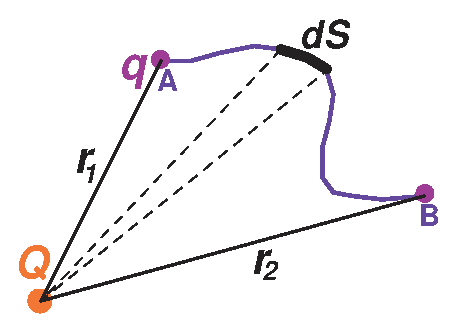
\includegraphics{GP015F20.eps}}
 \put(75,0){\makebox(0,0)[lb]{\parbox{115mm}{
 Пусть теперь путь из точки A в точку B тернист и извилист.
 Разобьем его на малые кусочки. На каждом таком кусочке $dS$ элементарная работа будет\vspace{-2mm}
 \begin{displaymath}
  \hspace{40mm}dA=\frac{Qq}{r^2}\cdot dr \vspace{-3mm}
 \end{displaymath}
 Полная же работа на участке $AB$ составит
 }}}
 \end{picture}\\
 \begin{displaymath}
  A=\int\limits_SdA=\int\limits_{r_1}^{r_2}\frac{Qq}{r^2}\cdot dr =
  Qq\int\limits_{r_1}^{r_2}\frac{dr}{r^2}=Qq\left(\frac1{r_1}-\frac1{r_2}\right)
  =q\left(\frac Q{r_1}-\frac Q{r_2}\right)
  %\vspace{-3mm}
 \end{displaymath}
 Как видим, работа по перемещению заряда $q$ пропорциональна величине этого заряда (это очевидно!) и разнсти неких величин, характеризующих НАЧАЛЬНОЕ и КОНЕЧНОЕ состояния. При этом, она НЕ ЗАВИСИТ от формы пути. Как мы видели в механике, такое свойство присуще ПОТЕН\-ЦИ\-АЛЬНЫМ силам.

 Введем функцию \underline{\bf потенциал}:\vspace{-4mm}
 \begin{displaymath}
  V=\frac Qr + C
 \end{displaymath}
 Тогда можно сказать, что работа по перемещению заряда на участке $AB$ равна произведению заряда на разность потенциалов в начальной и конечной точках:\vspace{-5mm}
 \begin{displaymath}
  A=q\cdot\left(V_A-V_B\right)
 \end{displaymath}
 Отсюда следует, что при перемещении по замкнутому контуру работа элек\-т\-ри\-чес\-ких сил = 0.\\
 \begin{picture}(190,30)(0,0)
 \put(120,0){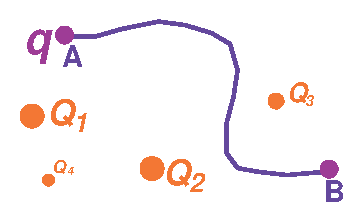
\includegraphics{GP015F21.eps}}
 \put(0,0){\makebox(0,0)[lb]{\parbox{115mm}{
 Если заряд $Q$, создающий поле, не один, то суммарная работа равна сумме работ, произведенных каждым из зарядов $Q_i$:
 }}}
 \end{picture}\\[-2mm]
 \begin{displaymath}
  A=q\left(V^{(1)}_A-V^{(1)}_B\right)+q\left(V^{(2)}_A-V^{(2)}_B\right)+\ldots+q\left(V^{(n)}_A-V^{(n)}_B\right)
 \end{displaymath}
 \begin{displaymath}
  V_A\equiv V^{(1)}_A+\ldots+V^{(n)}_A;\;\;\;\;V_B\equiv V^{(1)}_B+\ldots+V^{(n)}_B;\;\;\;\;  A=q\cdot\left(V_A-V_B\right)
 \end{displaymath}

 Любое заряженную систему можно разделить на $\infty$ число малых зарядов и говорить о потенциале, создаваемом системой. Поэтому забудем о зарядах $Q_i$ и будем оперировать ПОТЕНЦИАЛОМ ПОЛЯ.
 \begin{center}
 \fbox{\parbox{188mm}{\color{blue}\bf
 Разность потенциалов в двух точках измеряется работой, совершаемой силами поля при перемещении единичного положительного заряда из первой точки во вторую.
 }}
 \end{center}

Единицы измерения разности потенциалов:
\begin{itemize}
\item CGSE: когда при перемещении единичного заряда CGSE совершается работа в 1 эрг.
\item СИ: 1 Вольт = $\frac1{300}$ электростатической разности потенциалов. При пе\-ре\-ме\-ще\-нии 1 Кулона на 1 Вольт совершается работа в 1 Джоуль.
\end{itemize}

Что такое РАЗНОСТЬ потенциалов -- ясно. А что принять за сам ПО\-ТЕН\-ЦИАЛ?  В гравитации: потенциальная энергия = $mgh$,  потенциал = $gh$. Относительно ЧЕГО берется высота $h$? Уровня моря? Уровня стола?

Так же и в электростатике -- выбор "нуля" произволен. Если в формуле для потенциала точечного заряда
\begin{displaymath}
V=\frac Qr+C
\end{displaymath}
положить $C=0$:
\begin{displaymath}
V=\frac Qr
\end{displaymath}
то получим, что нулевым  потенциал становится при $r\rightarrow\infty$. Поэтому чаще всего за "нулевой" потенциал выбирается потенциал бесконечно удаленной точки.
 \begin{center}
 \fbox{\parbox{188mm}{\color{blue}\bf
 Потенциал данной точки поля численно равен работе, которую совершат силы поля при перемещении единичного положительного заряда из этой точки в бесконечно удаленную, потенциал которой принят за нулевой.
 }}
 \end{center}

На практике за "ноль" принимают потенциал земной поверхности.
\newpage

Рассмотрим теперь перемещение заряда $q$ в произвольном поле, каждая точка которого характеризуется какой-то напряженностью $\vec{E}$. Аналогично тому, как мы это проделали с полем точечного заряда $Q$, разобьем траекторию на участочки $dS$ и получим, что работа по перемещению  на каждом участке равна\vspace{-3mm}
\begin{displaymath}
dA= F \cos\alpha \;dS= q \;E\;\cos\alpha \; dS= q\;E_s\;dS=q\,\left(\vec{E}\cdot\vec{dS}\right)
\end{displaymath}
а вся работа на пути из A в B составит\vspace{-5mm}
\begin{displaymath}
\hspace{20mm}A=\int\limits_S dA=\int\limits_A^B q \;E_s\; dS.
\end{displaymath}
Поскольку она должна равняться $q(V_A-V_B)$, то получим:
\begin{displaymath}
\hspace{20mm}\int\limits_A^B E_s\; dS=V_A-V_B.
\end{displaymath}
Для замкнутой траектории\vspace{-9mm}
\begin{displaymath}
\oint\limits_S E_s\; dS=0,
\end{displaymath}
и это можно считать определением потенциального характера поля.
\\
 \begin{picture}(190,70)(0,0)
 \put(120,0){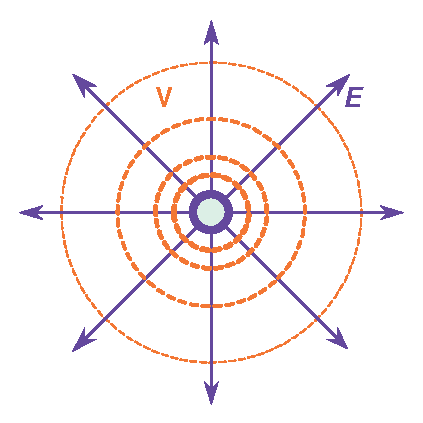
\includegraphics{GP015F22.eps}}
 \put(0,0){\makebox(0,0)[lb]{\parbox{115mm}{
Потенциал -- скалярная величина, меня\-ю\-ща\-я\-ся от точки к точке. Можно выделить места, где он одинаков -- \underline{\bf эквипотенциальные поверхности}. Для точечного, сферического или шарообразного зарядов это -- концентрические сферы (поскольку потенциал их имеет одинаковую форму: $V=Q/r$ -- и зависит только от $r$).
 }}}
 \end{picture}\\[-2mm]
 \begin{picture}(190,50)(0,0)
 \put(130,0){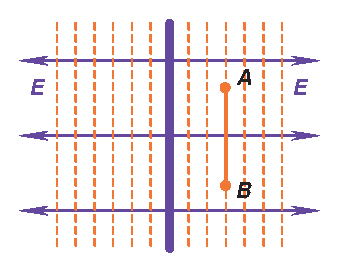
\includegraphics{GP015F23.eps}}
 \put(0,0){\makebox(0,0)[lb]{\parbox{125mm}{
 Для заряженной плоскости эквипотенциальные поверхности -- это плоскости $\parallel$ ей. При движении заряда вдоль такой поверхности (из А в В) напряженность движению $\Rightarrow$ работа =0, что и ожидалось (потенциал = const.)
 }}}
 \end{picture}\\[-2mm]

В общем случае: при малом перемещении в поле работа $dA=\left(\vec{F}\cdot\vec{dS}\right)=F\,\cos\alpha\,dS$. Чтобы она была =0, надо: $\cos\alpha$=0, то есть,$\vec{F}\perp\vec{dS}$. Эк\-ви\-по\-тен\-ци\-аль\-ные поверхности всегда $\perp$ напряженности поля.

Если поле создано положительным зарядом, то силы толкают наш {\em проб\-ный} заряд $+q$ прочь, к $\infty$, производя при этом положительную работу, и потенциал тоже положителен и убывает с радиусом.

Если же преобладают отрицательные заряды, то они будут наш {\em проб\-ный} заряд $+q$ притягивать, и для удаления его на $\infty$ уже нам придется совершать работу против поля, потенциал является отрицательным, образуя потенциальную яму.\\
 \begin{picture}(190,155)(0,0)
 \put(20,0){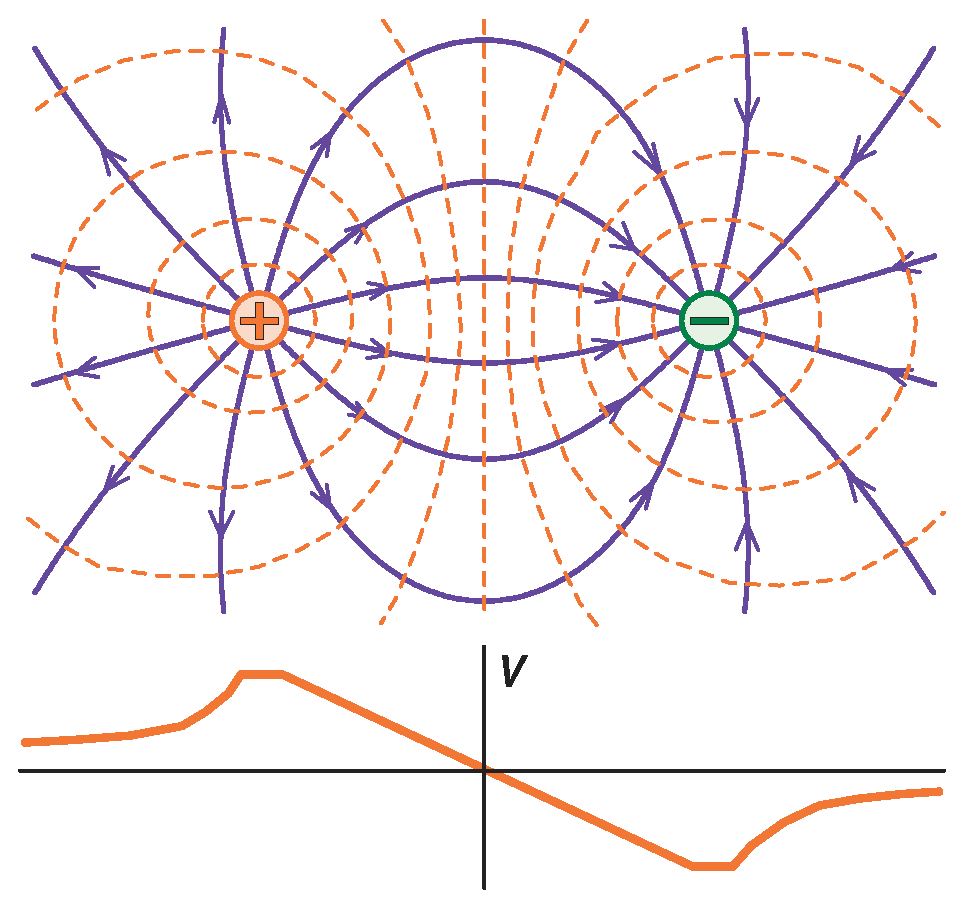
\includegraphics{GP015F24.eps}}
 \end{picture}
 \newpage
 \noindent
 \begin{picture}(190,40)(0,0)
 \put(135,0){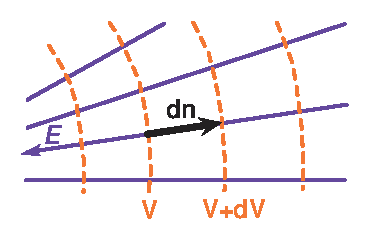
\includegraphics{GP015F25.eps}}
 \put(0,0){\makebox(0,0)[lb]{\parbox{130mm}{
 В какой-то точке проведем нормаль $\vec{n}$ к эквипотенциальной поверхности в сто\-ро\-ну воз\-рас\-та\-ния потенциала. Поскольку напряженность поля всегда $\perp$ этой по\-вер\-х\-но\-с\-ти, то она $\parallel$ нормали. Если двинуть пробный заряд $+q$ вдоль нормали на
 }}}
 \end{picture}\\[-1mm]
малое расстояние $dn$, то работа поля составит $A=q\left(\vec{E}\cdot\vec{dn}\right)=q\,E\,dn$. Но, с другой стороны, эта работа должна быть
 \begin{displaymath}
  A=q\cdot(V_1-V_2)=q\cdot\left[V_1-(V_1+dV)\right]=-q\,dV
 \end{displaymath}
Отсюда получаем, что
 \begin{displaymath}
  E=-\frac{dV}{dn}=q\cdot\left[V_1-(V_1+dV)\right]=-q\,dV
 \end{displaymath}
Вообще-то, нормаль к эквипотенциальной поверхности -- это градиент. Тогда
 \begin{displaymath}
  E=-\vec{\rm grad}\, V = -\vec{\nabla} V
 \end{displaymath}
{\small\color{blue}  \underline{\bf шпаргалка:} {\em Если есть скалярная функция $U(x,y,z)$, то ее градиент $\vec{\nabla}U$ -- это вектор с составляющими:
 \begin{displaymath}
  \frac{\partial U}{\partial x},\;\;\;\;
  \frac{\partial U}{\partial y},\;\;\;\;
  \frac{\partial U}{\partial z}\vspace{-3mm}
 \end{displaymath}
}}
 \begin{displaymath}
  E_x=-\frac{\partial V}{\partial x},\;\;\;\;  E_y=-\frac{\partial V}{\partial y},\;\;\;\;  E_z=-\frac{\partial V}{\partial z}\vspace{3mm}
 \end{displaymath}
 \begin{picture}(190,20)(0,0)
 \put(100,0){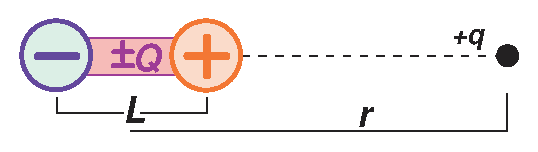
\includegraphics{GP015F26.eps}}
 \put(0,0){\makebox(0,0)[lb]{\parbox{90mm}{
\underline{\bf Задачка:} Найти поле на оси диполя вдали от него ($r\gg L$).
 }}}
 \end{picture}\\[-1mm]
\underline{\bf 2 Решения} ("в лоб" и через потенциал):
 \begin{displaymath}
 1)\;\;\;\;
  E=\frac{Q}{r_+^2}-\frac{Q}{r_-^2}=Q\frac{r_-^2-r_+^2}{r_+^2\,r_-^2}=Q\frac{(r_--r_+)(r_-+r_+)}{r_+^2\,r_-^2}
  \simeq Q\frac{L(2r)}{r^4}=\frac{2QL}{r^3}
 \end{displaymath}
 \begin{displaymath}
 2)\;\;\;\; V=\;\frac{-Q}{r_-}\;+\;\frac{+Q}{r_+}\;\;=\;\;Q\,\frac{r_--r_+}{r_+r_-}\;\;=\;\;Q\,\frac{L}{r_+r_-}\;\;\simeq
  \;\;Q\,\frac{L}{r^2}\hspace{30mm}
 \end{displaymath}
 \begin{displaymath}
  E\;\;=\;\; -\vec{\nabla} V\;\;=\;\;-\frac{\partial V}{\partial r}\;\;=\;\;\frac{2QL}{r^3}
 \end{displaymath}
 \begin{picture}(190,40)(0,0)
 \put(120,0){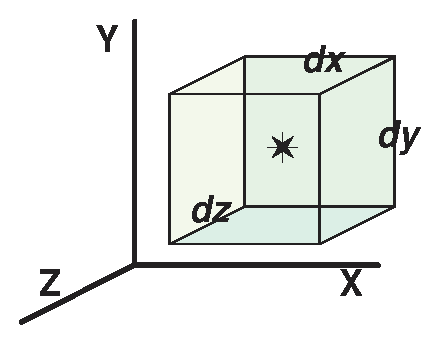
\includegraphics{GP015F27.eps}}
 \put(0,0){\makebox(0,0)[lb]{\parbox{125mm}{
Пусть в пространстве как-то распределены заряды с плотностью $\rho(x,y,z)$. Выделим там маленький кубик $dx\times dy\times dz$. Напряженность поля в центре = $\vec{E}$ с составляющими $E_x$, $E_y$ и $E_z$. Значение $E_x$ на левой грани будет\vspace{-3mm}
 \begin{displaymath}
  E_x^L\;\;=\;\; E_x-\frac{\partial E_x}{\partial x}\cdot\frac{dx}2,
 \end{displaymath}
 }}}
 \end{picture}\\[-1mm]
на правой -- \vspace{-3mm}
 \begin{displaymath}
  \hspace{-60mm}E_x^R\;\;=\;\; E_x+\frac{\partial E_x}{\partial x}\cdot\frac{dx}2,
 \end{displaymath}
на нижней и верхней --\vspace{-3mm}
 \begin{displaymath}
  E_y^D\;\;=\;\; E_y-\frac{\partial E_y}{\partial y}\cdot\frac{dy}2,\hspace{20mm}
  E_y^U\;\;=\;\; E_y+\frac{\partial E_y}{\partial y}\cdot\frac{dy}2,
 \end{displaymath}
а на задней и передней --\vspace{-2mm}
 \begin{displaymath}
  E_z^B\;\;=\;\; E_z-\frac{\partial E_z}{\partial z}\cdot\frac{dz}2,\hspace{20mm}
  E_z^F\;\;=\;\; E_z+\frac{\partial E_z}{\partial z}\cdot\frac{dz}2.
 \end{displaymath}
Поток напряженности через правую грань равен
 \begin{displaymath}
  dN^R=E_x^R\cdot (dy\,dz)= E_x\,dy\,dz+\frac{\partial E_x}{\partial x}\cdot\frac12\,dx\,dy\,dz.
 \end{displaymath}
Для левой грани нормаль направлена \underline{\bf против} оси $\vec{X}$, поэтому нормальная составляющая напряженности $\vec{E}$ для этой грани равна не $E_x^L$, а $-E_x^L$, и поток через нее будет\vspace{-3mm}
 \begin{displaymath}
  dN^L=-E_x^L\cdot (dy\,dz)= -E_x\,dy\,dz+\frac{\partial E_x}{\partial x}\cdot\frac12\,dx\,dy\,dz.
 \end{displaymath}
Суммарный поток через левую и правую грани кубика =
 \begin{displaymath}
  dN^{LR}=dN^L+dN^R=\frac{\partial E_x}{\partial x}\,dx\,dy\,dz.
 \end{displaymath}
Аналогично, суммарный поток через нижнюю и верхнюю грани =
 \begin{displaymath}
  dN^{DU}=dN^D+dN^U=\frac{\partial E_y}{\partial y}\,dx\,dy\,dz,
 \end{displaymath}
а через заднюю и переднюю --\vspace{-3mm}
 \begin{displaymath}
  dN^{BF}=dN^B+dN^F=\frac{\partial E_z}{\partial z}\,dx\,dy\,dz.
 \end{displaymath}
Полный заряд, находящийся внутри кубика: $q=\rho\,dx\,dy\,dz$, и по теореме О-Г получаем
 \begin{displaymath}
  \frac{\partial E_x}{\partial x}+\frac{\partial E_y}{\partial y}+\frac{\partial E_z}{\partial z}=4\pi\rho.
 \end{displaymath}
{\small\color{blue}  \underline{\bf шпаргалка:} {\em Если есть векторная функция $\vec{F}(x,y,z)$, то ее дивергенция div $\vec{F}$ -- это сумма производных от составляющих функции по осям:
 \begin{displaymath}
  {\rm div}\,\vec{F}=\frac{\partial F_x}{\partial x}+
  \frac{\partial F_y}{\partial y}+
  \frac{\partial F_z}{\partial z}\vspace{-3mm}
 \end{displaymath}
}}
 \begin{displaymath}
  {\rm div}\,\vec{E}=4\pi\rho
 \end{displaymath}
Если вспомнить, что напряженность выражается через потенциал как
 \begin{displaymath}
  E_x=-\frac{\partial V}{\partial x},\;\;\;\;  E_y=-\frac{\partial V}{\partial y},\;\;\;\;  E_z=-\frac{\partial V}{\partial z},\vspace{3mm}
 \end{displaymath}
то дифференцируя это второй раз, получим:
 \begin{displaymath}
  \frac{\partial^2V}{\partial x^2}+\frac{\partial^2V}{\partial y^2}+\frac{\partial^2V}{\partial z^2}=-4\pi\rho.
 \end{displaymath}
{\small\color{blue}  \underline{\bf шпаргалка:} {\em Если есть скалярная функция $U(x,y,z)$, то сумма ее вторых производных по осям обозначается как $\triangle U$, где $\triangle$ -- это оператор Лапласа
 \begin{displaymath}
  \triangle=\frac{\partial^2}{\partial x^2}+
  \frac{\partial^2}{\partial y^2}+
  \frac{\partial^2}{\partial z^2}\vspace{-3mm}
 \end{displaymath}
}}
 \begin{displaymath}
  \triangle V=-4\pi\rho.
 \end{displaymath}
\vspace{5mm}

\underline{\bf Проводник в электрическом поле.}\\
 \begin{picture}(190,25)(0,0)
 \put(140,0){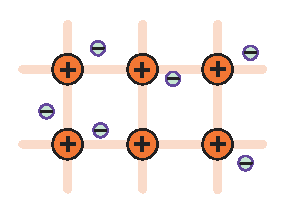
\includegraphics{GP015F28.eps}}
 \put(0,0){\makebox(0,0)[lb]{\parbox{135mm}{
 Как уже говорилось, проводник имеет свободные электроны, которые могут по нему перемещаться.
 Если бы на них действовало поле $\neq0$, то они бы дви-
 }}}
 \end{picture}\\
 гались, меняя это поле до тех пор, пока оно не стало бы =0. Коль скоро мы изучаем электро\underline{СТАТИКУ}, то это значит: ничто \underline{не движется}, и $\Rightarrow$ поле внутри проводника =0. Если мысленно выделить {\bf внутри} проводника некий объем, то, поскольку напряженность везде =0, то и ее поток через поверхность =0, и по теореме О-Г нескомпенсированные заряды внутри =0.
\begin{center}
\fbox{\parbox{185mm}{\color{blue}\bf Заряды в заряженном проводнике $\exists$ лишь на его поверхности.}}\\[1mm]
Весь проводник имеет один и тот же потенциал.
\end{center}







\end{document}
